\chapter{Apresentação de EVA}

Neste capítulo, serão apresentadas as principais funcionalidades de EVA, já em funcionamento, na plataforma de mensagens instantâneas Telegram. É válido salientar que por motivos de segurança e integridade, como estão sendo utilizados dados reais dos alunos vinculados ao EV.G, em algumas figuras foram postas tarjas pretas sob informações que são consideradas pessoais do usuário.

\section{Introdução}

Ao inicializar uma conversa com EVA, ela dará as boas-vindas e irá solicitar ao usuário que o mesmo se autentique, fornecendo o CPF ou o e-mail cadastrado na EV.G. Na Figura \ref{cap:04:fig:apresentacao-boas-vindas} é demonstrada tal situação.

\begin{figure}[htb!]
    \centering
    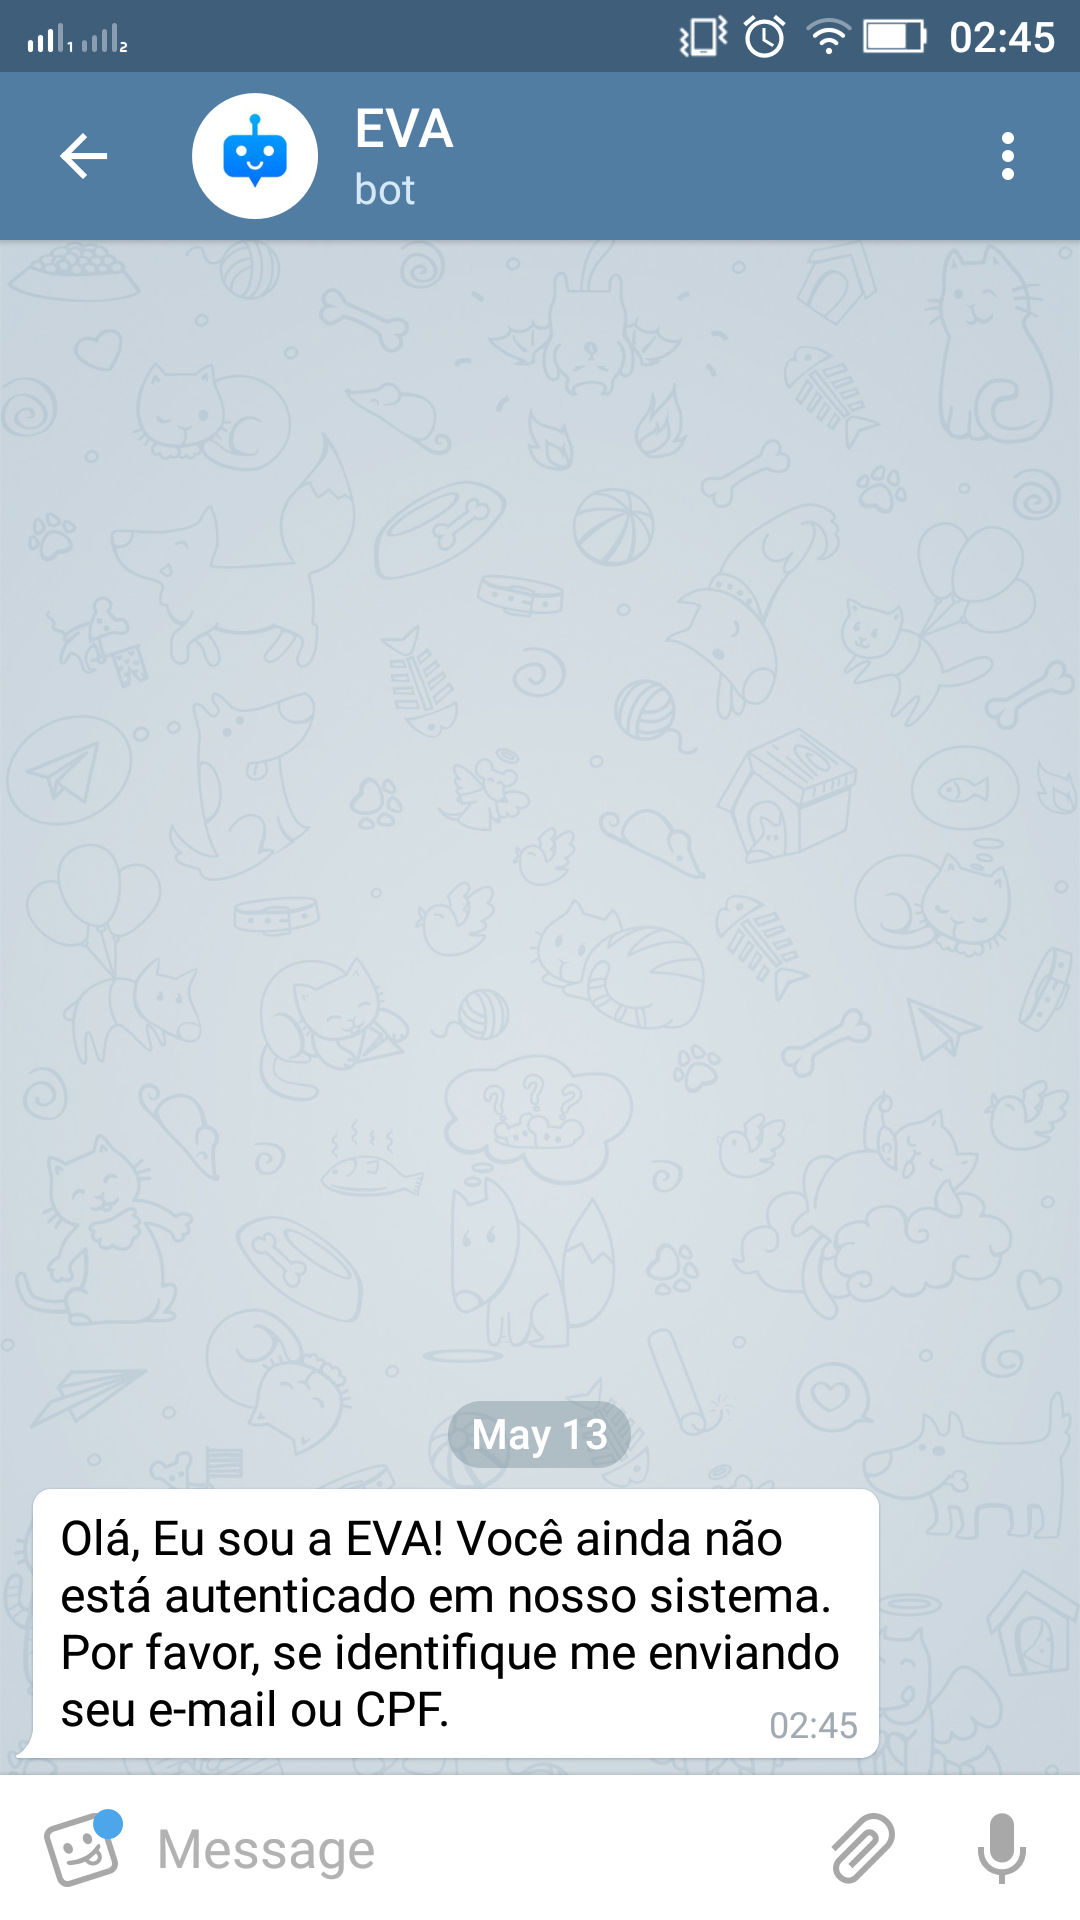
\includegraphics[width=0.2\linewidth]{src/imagens/apresentacao-boas-vindas.png}
    \caption{EVA - Boas-vindas} Fonte: Elaborado pelo autor (2018)
    \label{cap:04:fig:apresentacao-boas-vindas}
\end{figure}

\section{Autenticação}
O usuário poderá se autenticar para usufruir das funcionalidades mais sofisticadas de EVA. Para essa funcionalidade existem dois cenários possíveis: O de falha e o de sucesso na autenticação.

\subsection{Falha na autenticação}
Caso as credenciais fornecidas pelo usuário não estiverem corretas, EVA irá enviar uma mensagem dizendo que os dados não conferem e irá solicitar que o usuário informe o CPF ou o e-mail novamente. Se o usuário tentar se autenticar sem sucesso por três vezes consecutivas, o sistema irá bloqueá-lo por 24 horas e o \textit{chatbot} irá informar tal acontecimento ao usuário. Essas situações são apresentadas na Figura \ref{cap:04:fig:apresentacao-autenticação-falha}.

\begin{figure}[htb!]
    \centering
    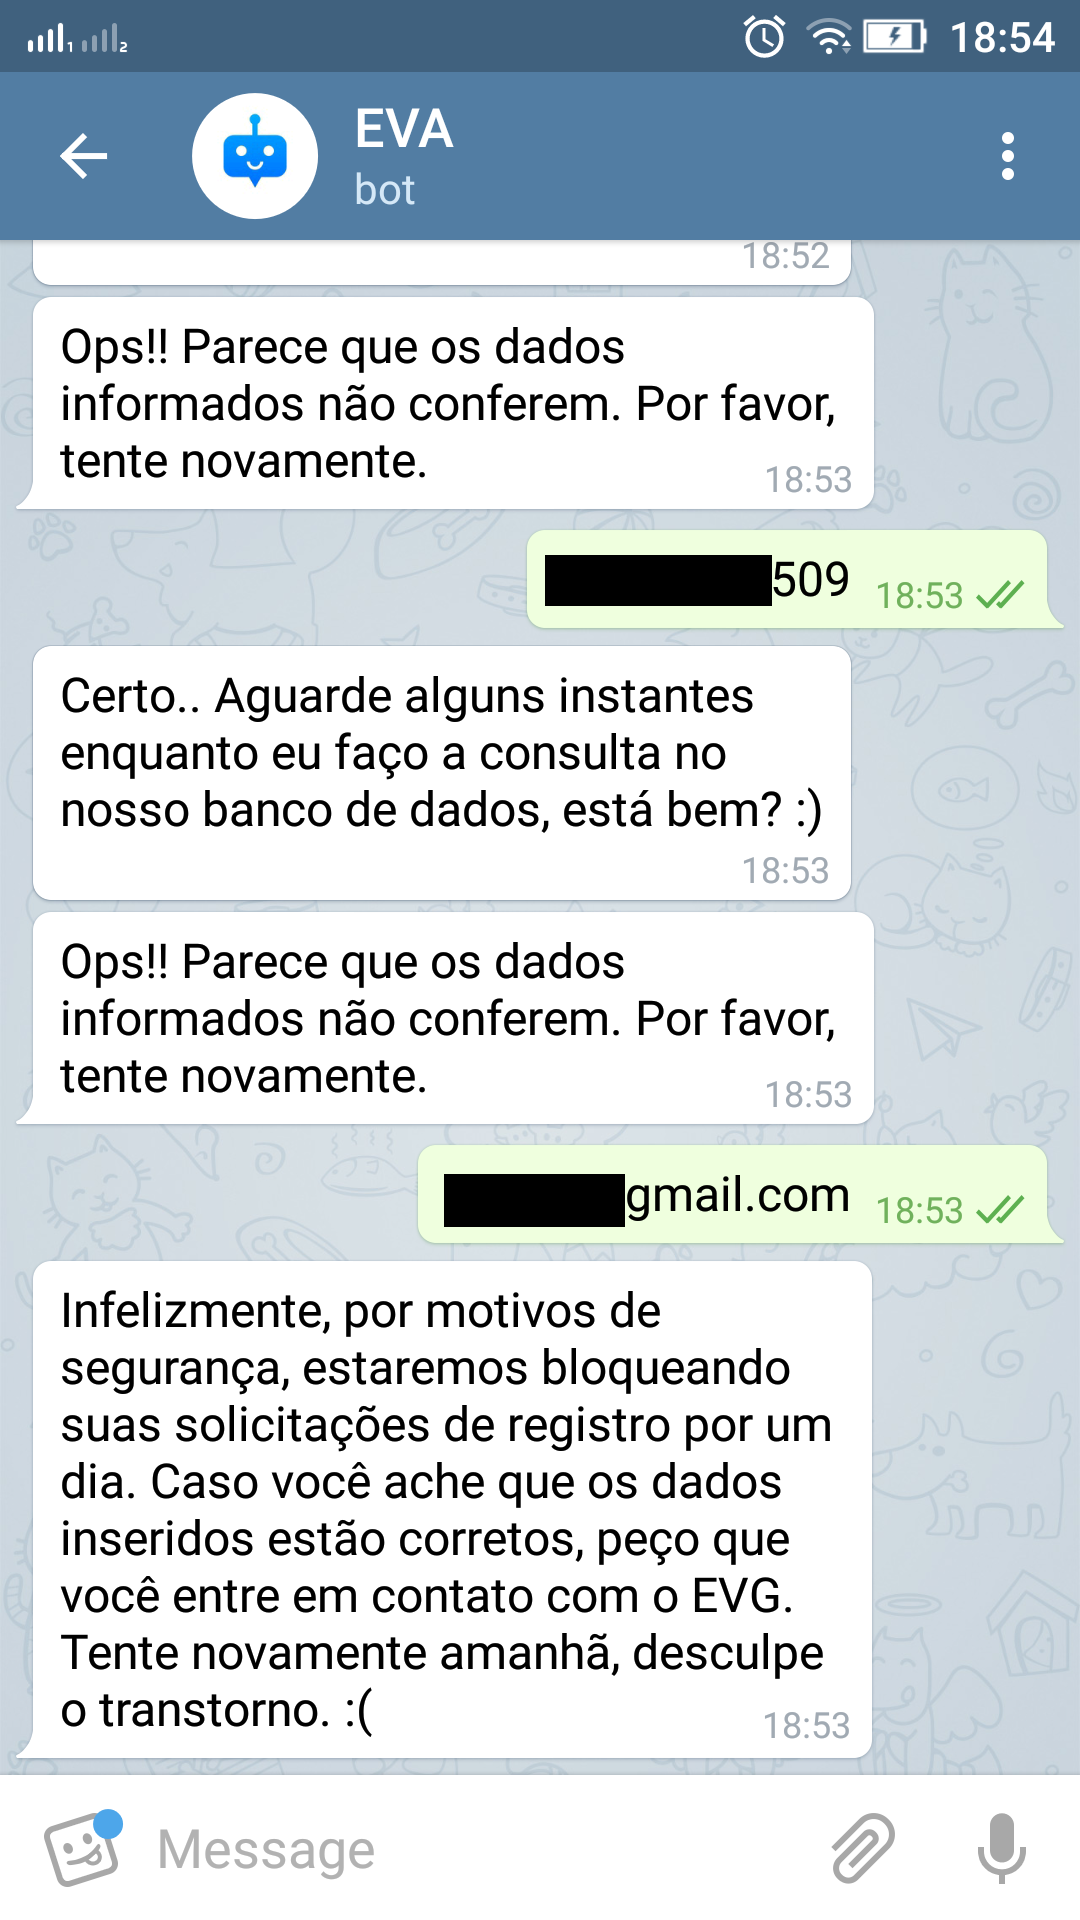
\includegraphics[width=0.2\linewidth]{src/imagens/apresentacao-autenticacao-falha.png}
    \caption{EVA - Bloqueio de usuário} Fonte: Elaborado pelo autor (2018)
    \label{cap:04:fig:apresentacao-autenticação-falha}
\end{figure}

\subsection{Sucesso na autenticação}
O aluno conseguiu se autenticar com sucesso no sistema e passará a ter acesso às funcionalidades mais sofisticadas de EVA. Na Figura \ref{cap:04:fig:apresentacao-autenticação-sucesso} este caso é apresentado.

\begin{figure}[htb!]
    \centering
    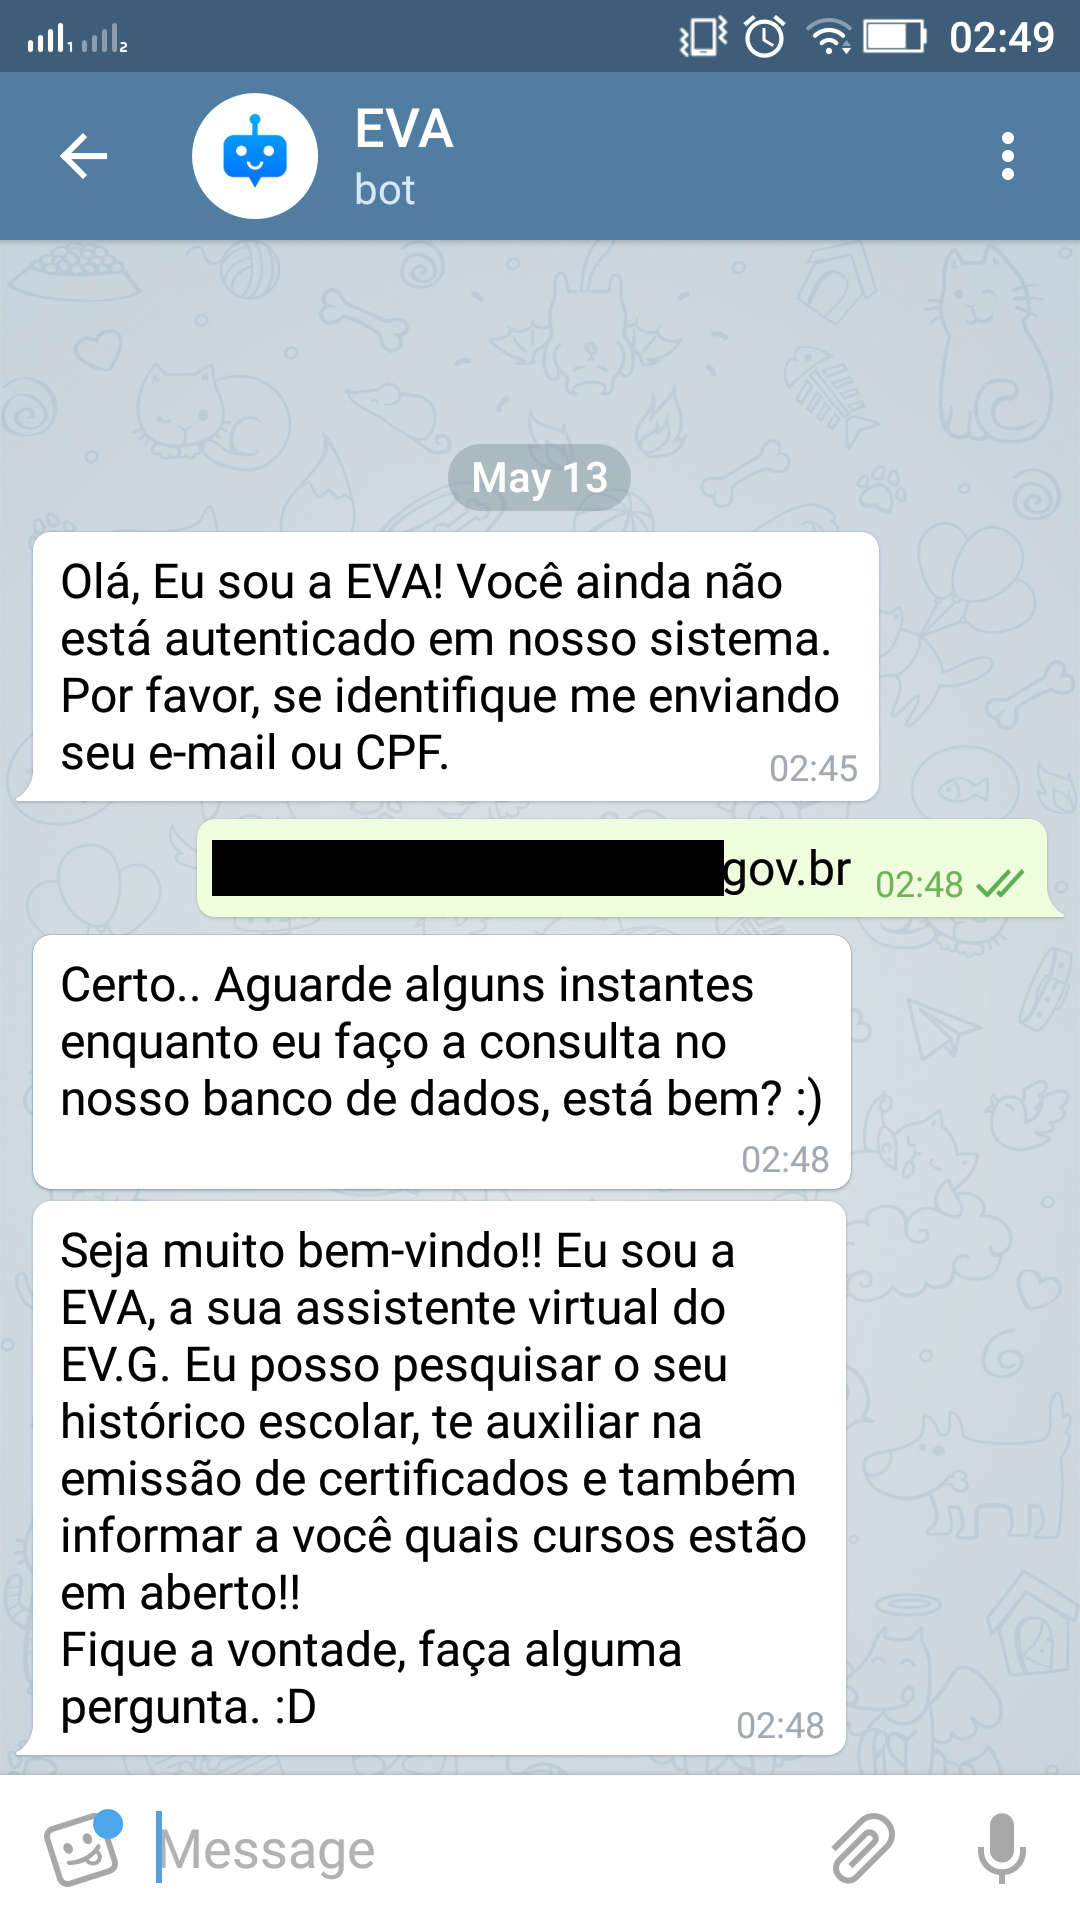
\includegraphics[width=0.2\linewidth]{src/imagens/apresentacao-autenticacao-sucesso.png}
    \caption{EVA - Autenticação realizada com sucesso} Fonte: Elaborado pelo autor (2018)
    \label{cap:04:fig:apresentacao-autenticação-sucesso}
\end{figure}

\section{Dialogando com EVA}

Por se tratar de um \textit{chatbot} de domínio amplo, EVA compreende algumas nuances nas mensagens enviadas por um aluno, compreendendo quais funcionalidades ele deseja utilizar e também sabendo quando um usuário está a cumprimentando, xingando e até mesmo quando recebe mensagens de afeto, como mostrada na Figura \ref{cap:04:fig:apresentacao-dialogos}.

\begin{figure}[htb!]
    \centering
    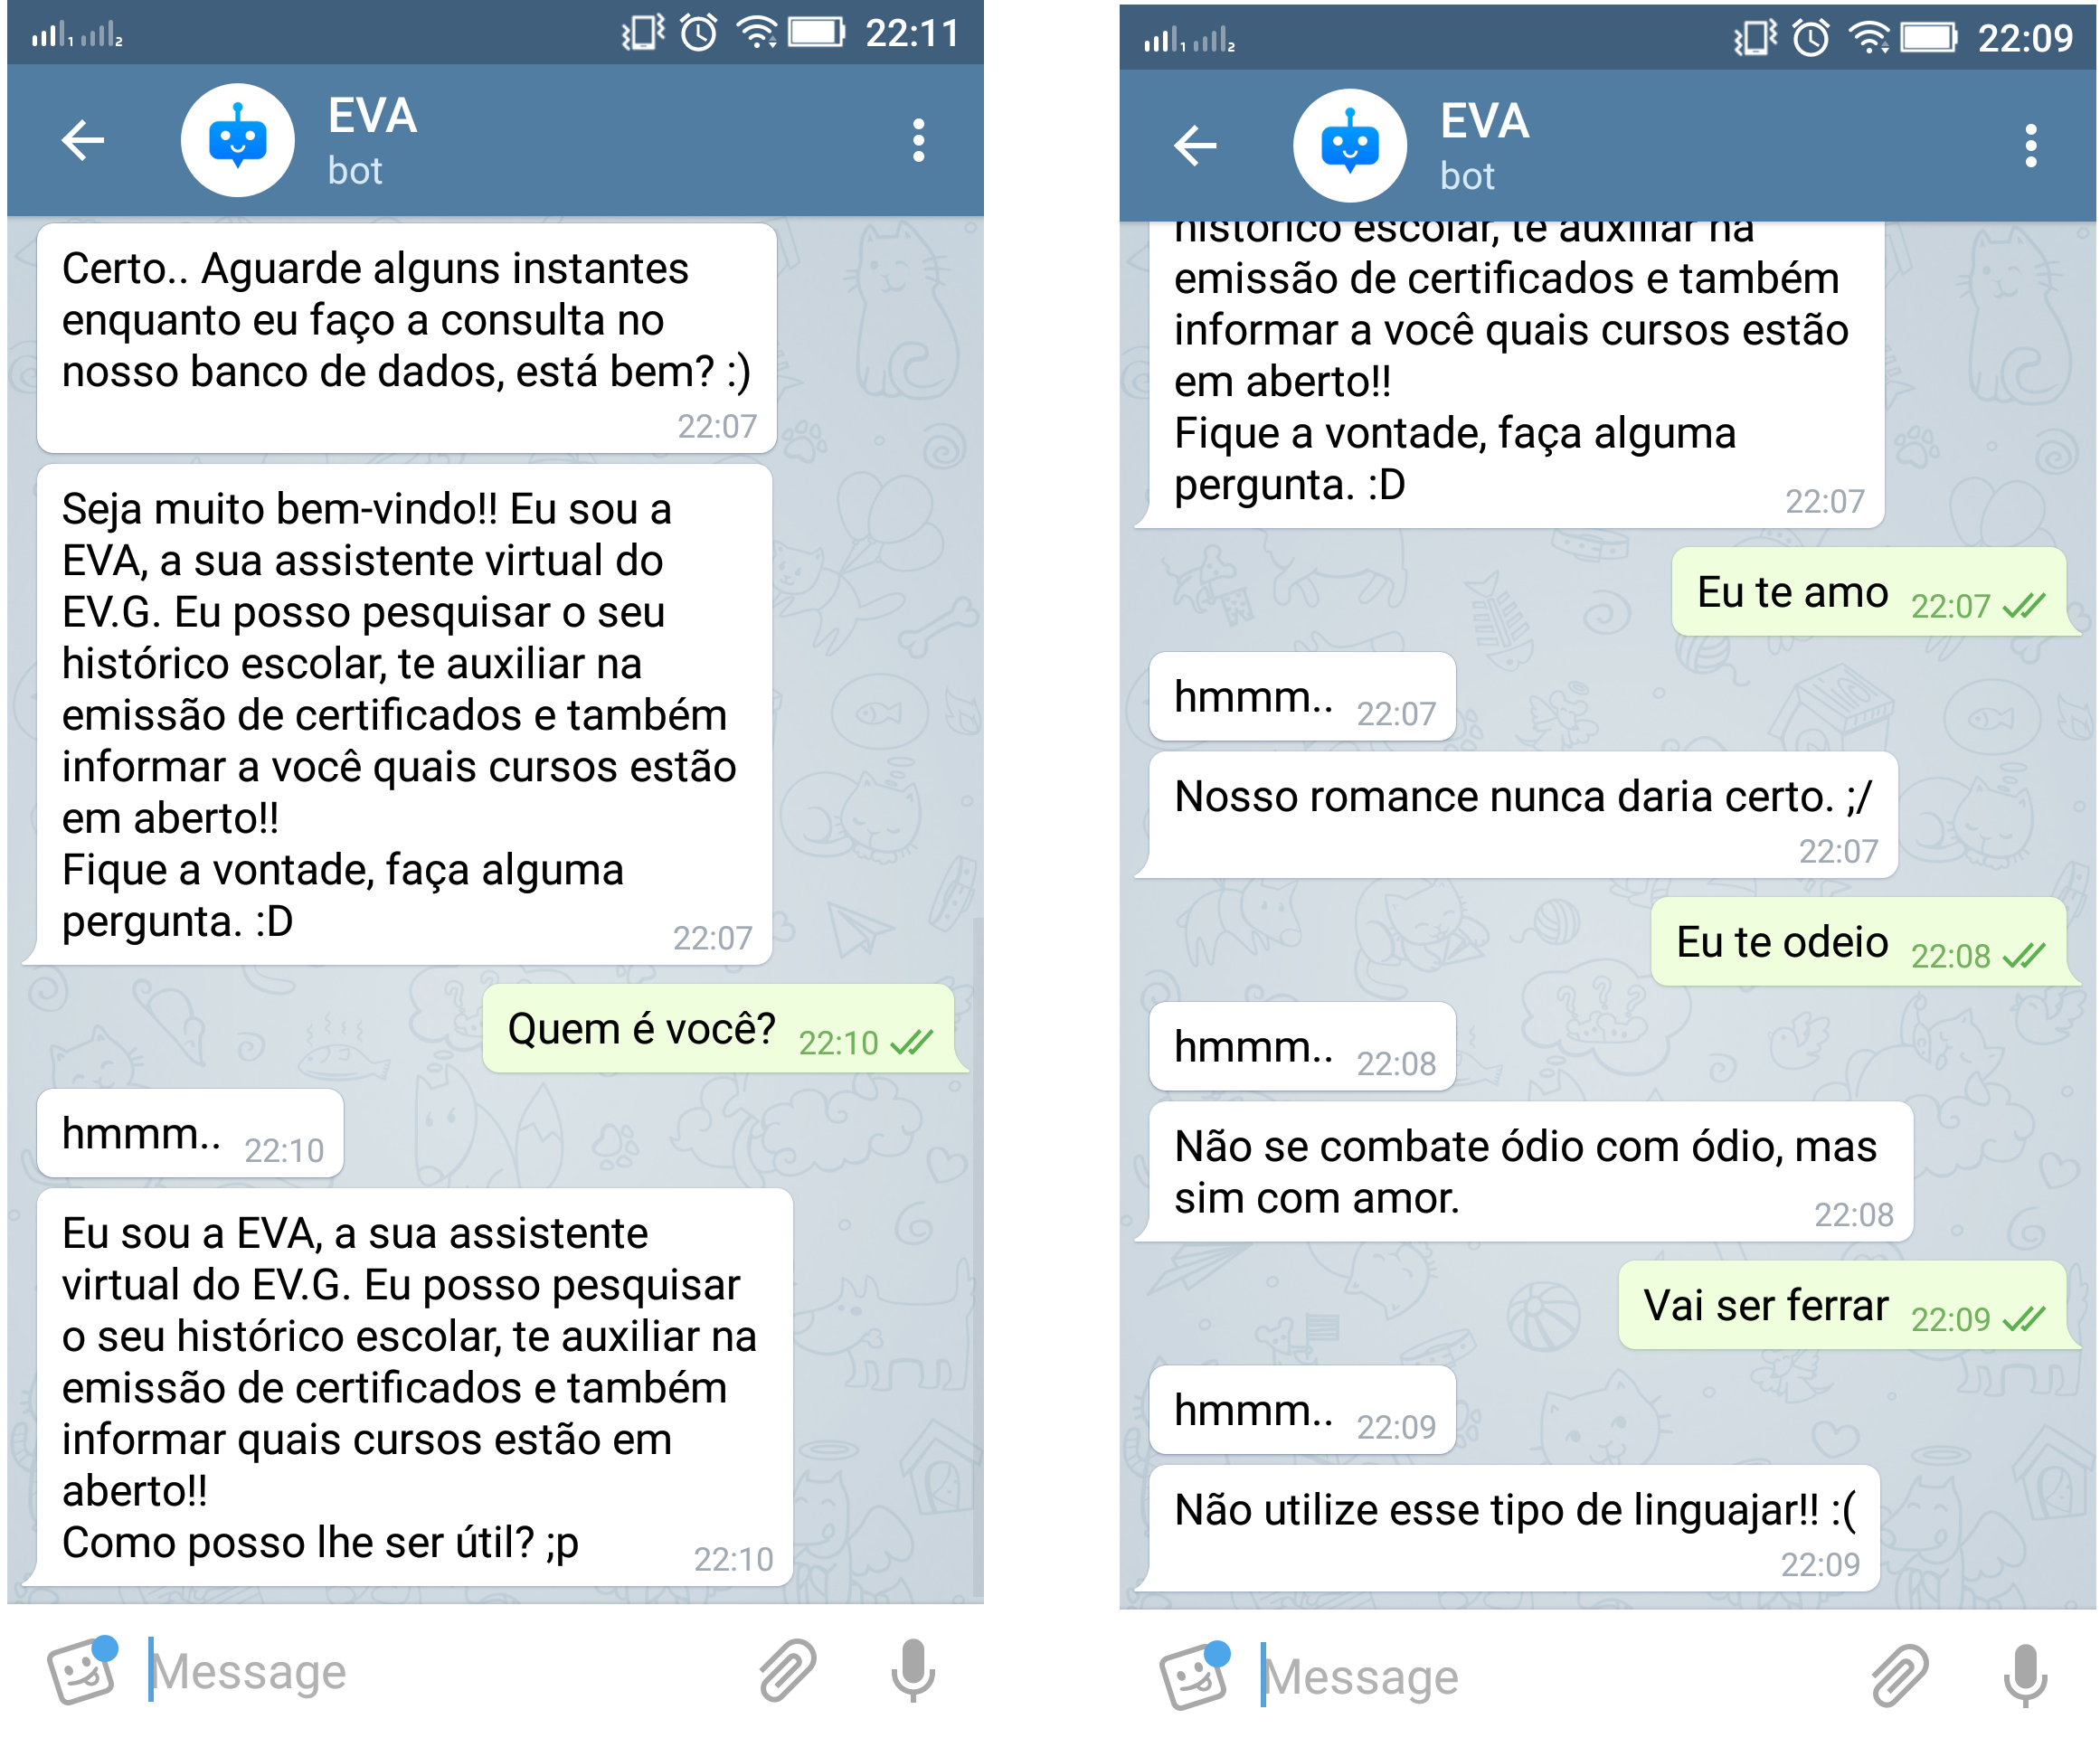
\includegraphics[width=0.4\linewidth]{src/imagens/apresentacao-dialogos.png}
    \caption{EVA - Dialogando} Fonte: Elaborado pelo autor (2018)
    \label{cap:04:fig:apresentacao-dialogos}
\end{figure}

\section{Visualizando o histórico escolar completo}

O aluno pode consultar o seu histórico escolar completo de maneira rápida e prática, como apresentado na Figura \ref{cap:04:fig:apresentacao-visualizar-historico}.

\begin{figure}[htb!]
    \centering
    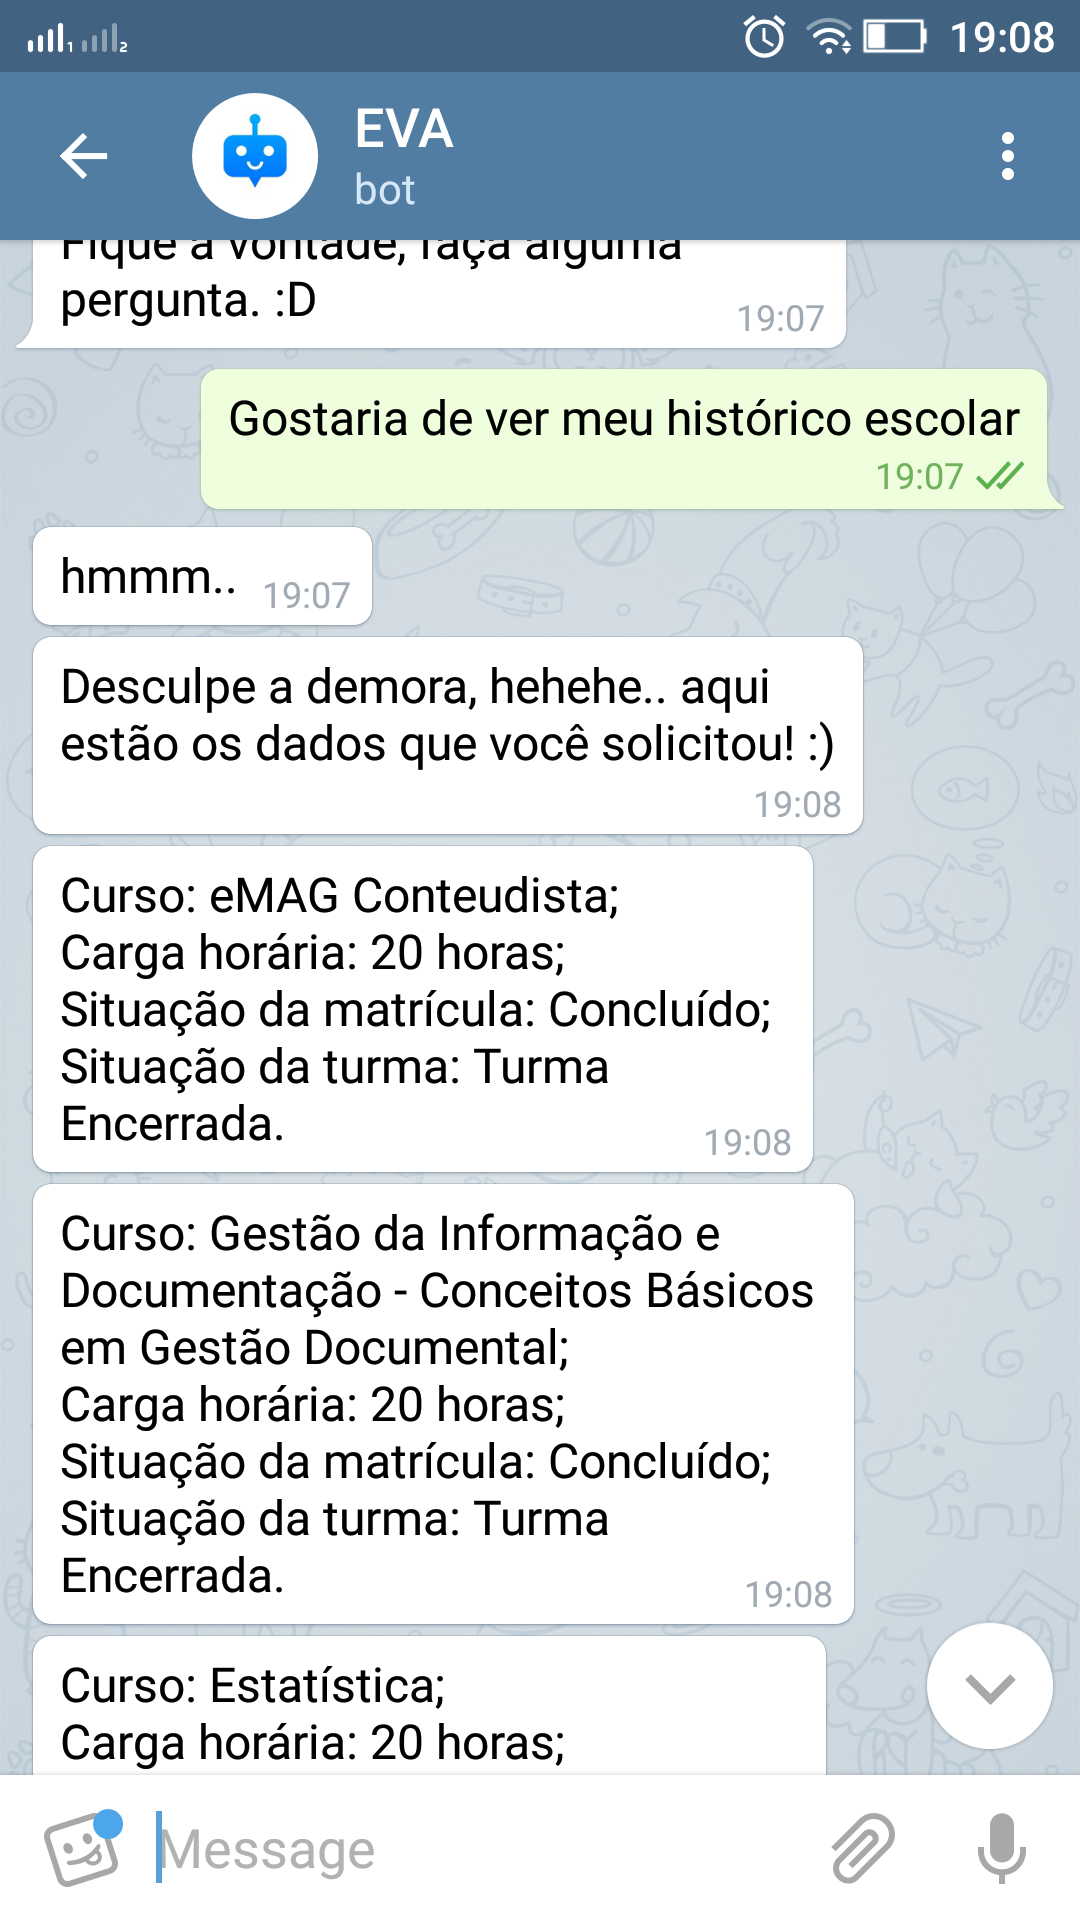
\includegraphics[width=0.2\linewidth]{src/imagens/apresentacao-visualizar-historico.png}
    \caption{EVA - Visualizando histórico escolar completo} Fonte: Elaborado pelo autor (2018)
    \label{cap:04:fig:apresentacao-visualizar-historico}
\end{figure}

\section{Auxiliando na emissão de certificados}

Se o aluno desejar, EVA pode auxiliá-lo na emissão de certificados dos cursos concluídos por ele, como exibido na Figura \ref{cap:04:fig:apresentacao-auxilio-certificados}.

\begin{figure}[htb!]
    \centering
    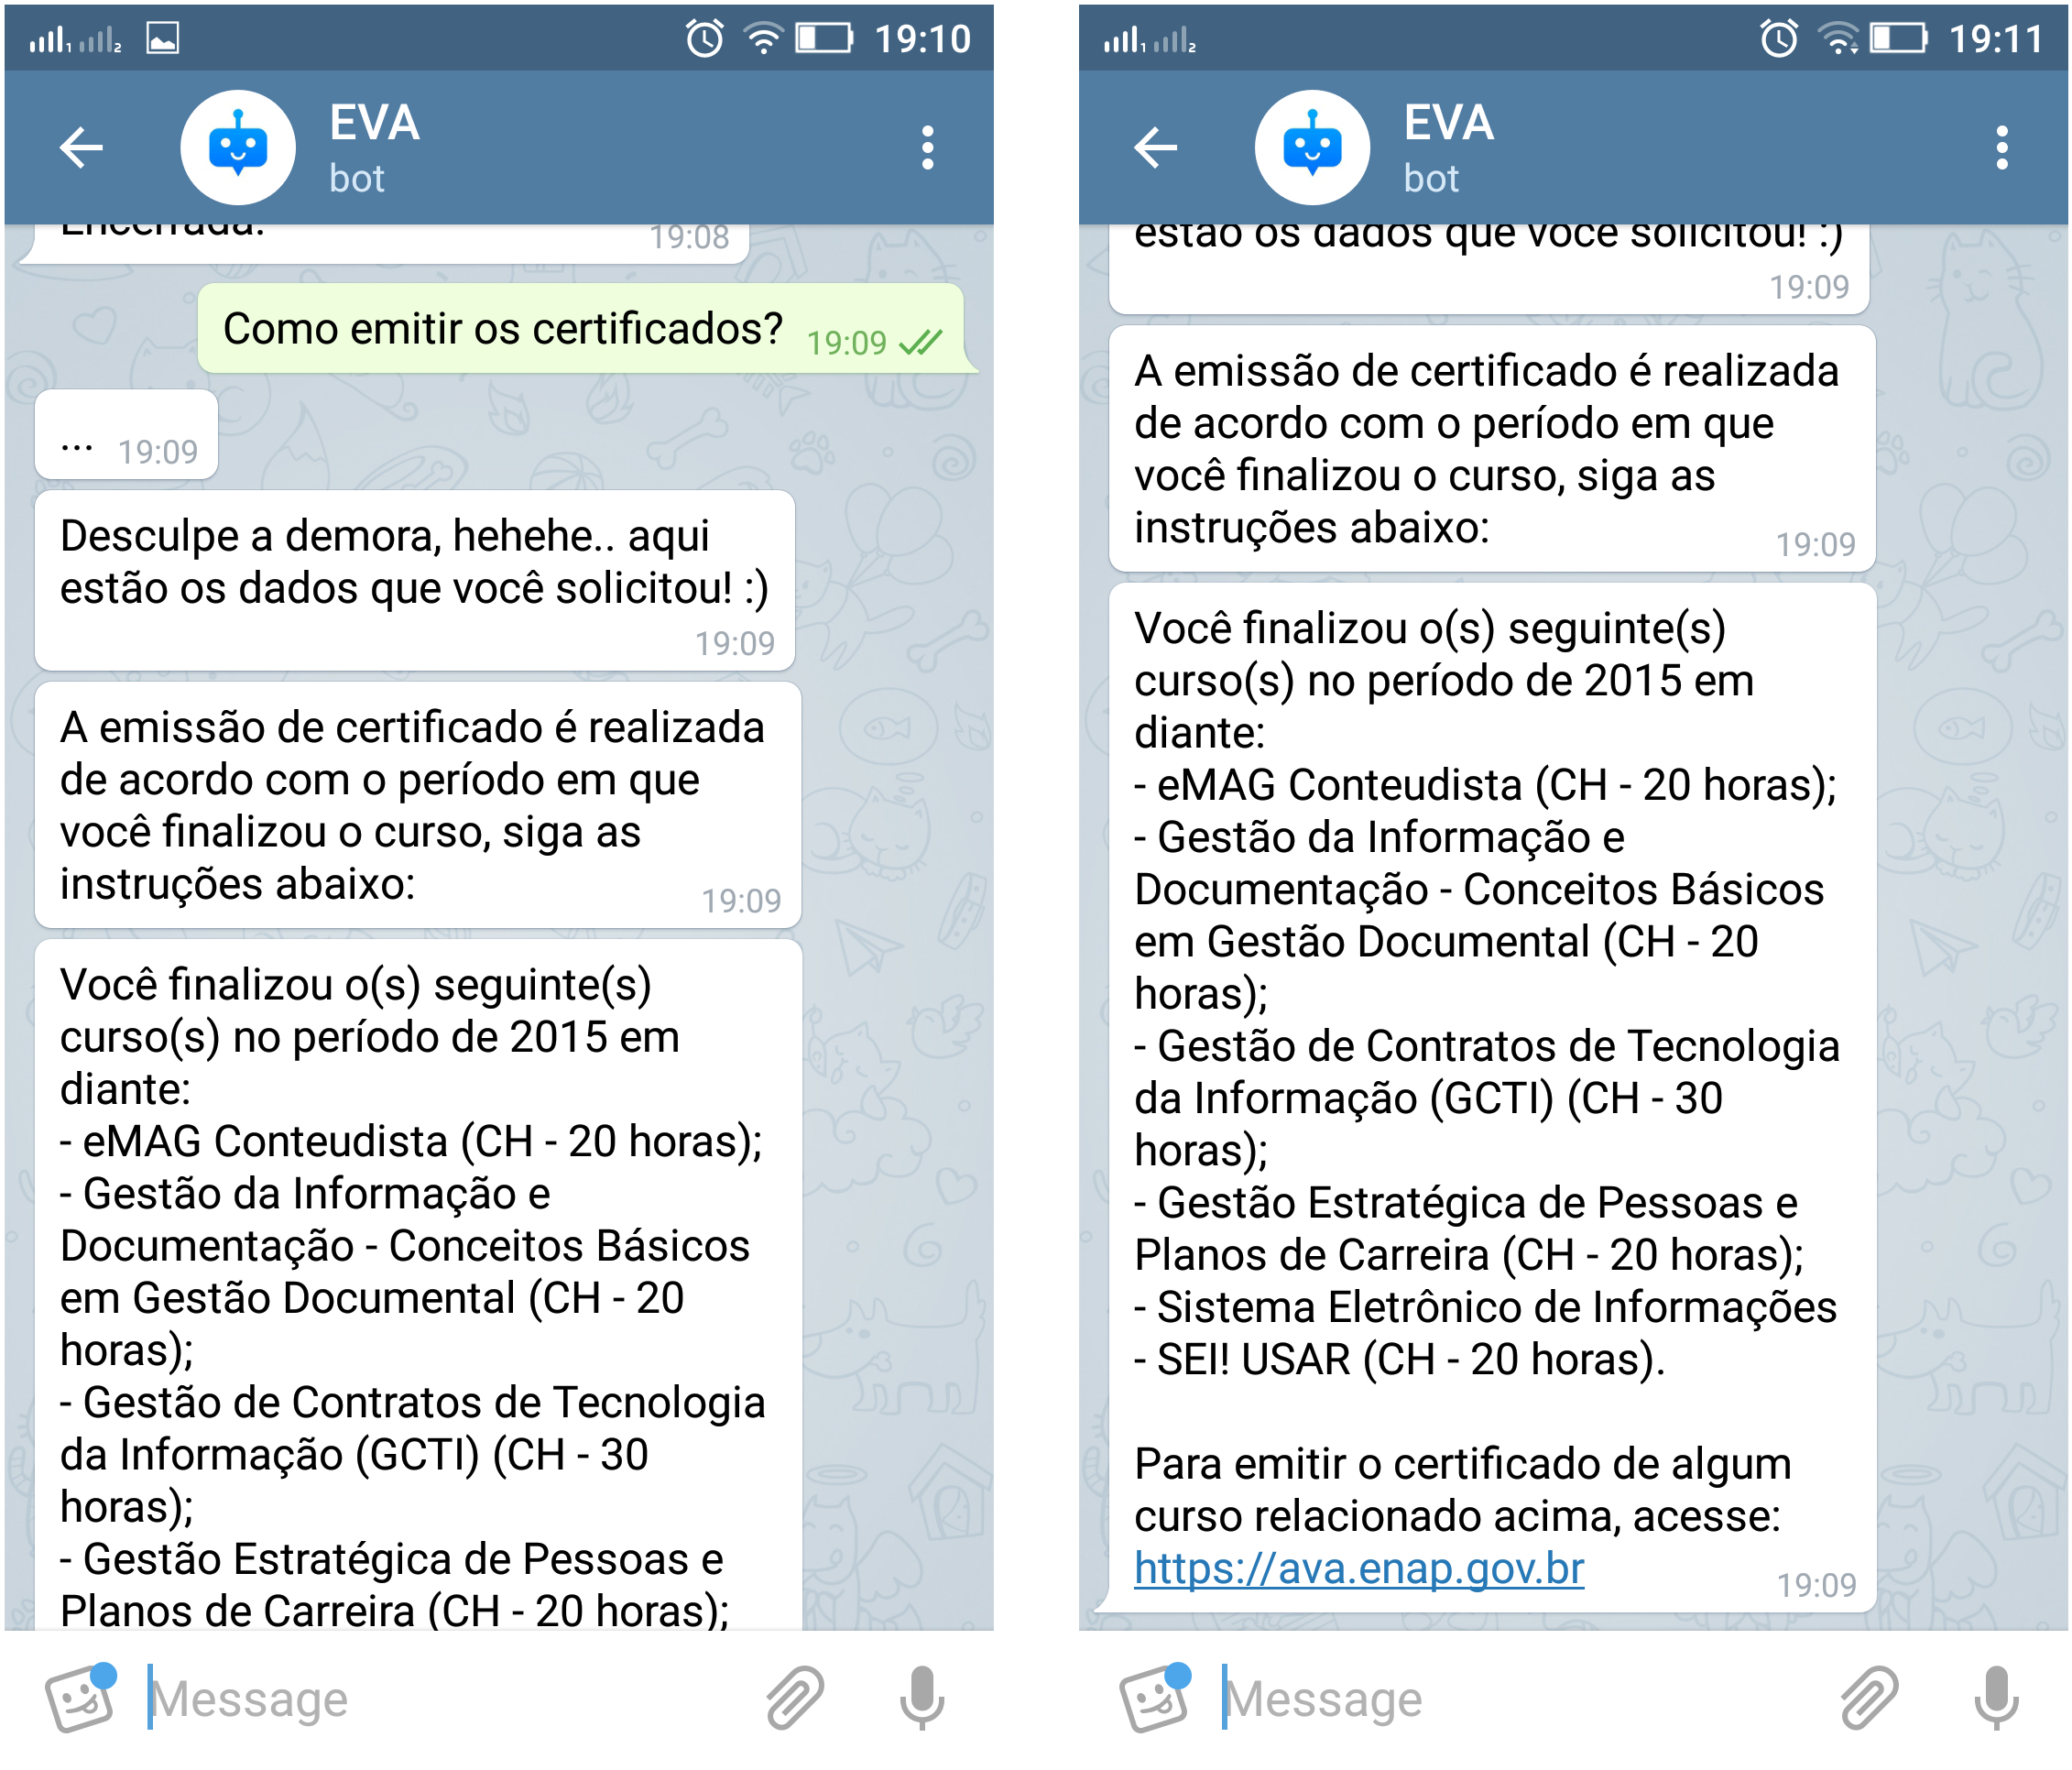
\includegraphics[width=0.4\linewidth]{src/imagens/apresentacao-auxilio-certificados.png}
    \caption{EVA - Auxiliando na emissão de certificados} Fonte: Elaborado pelo autor (2018)
    \label{cap:04:fig:apresentacao-auxilio-certificados}
\end{figure}

\section{Visualizando inscrições de cursos abertos}

Caso o aluno esteja em dúvida sobre quais inscrições de cursos estão em aberto, com uma mensagem de texto ele terá acesso a essas informações, como apresentado na Figura \ref{cap:04:fig:apresentacao-inscricoes-aberto}.

\begin{figure}[htb!]
    \centering
    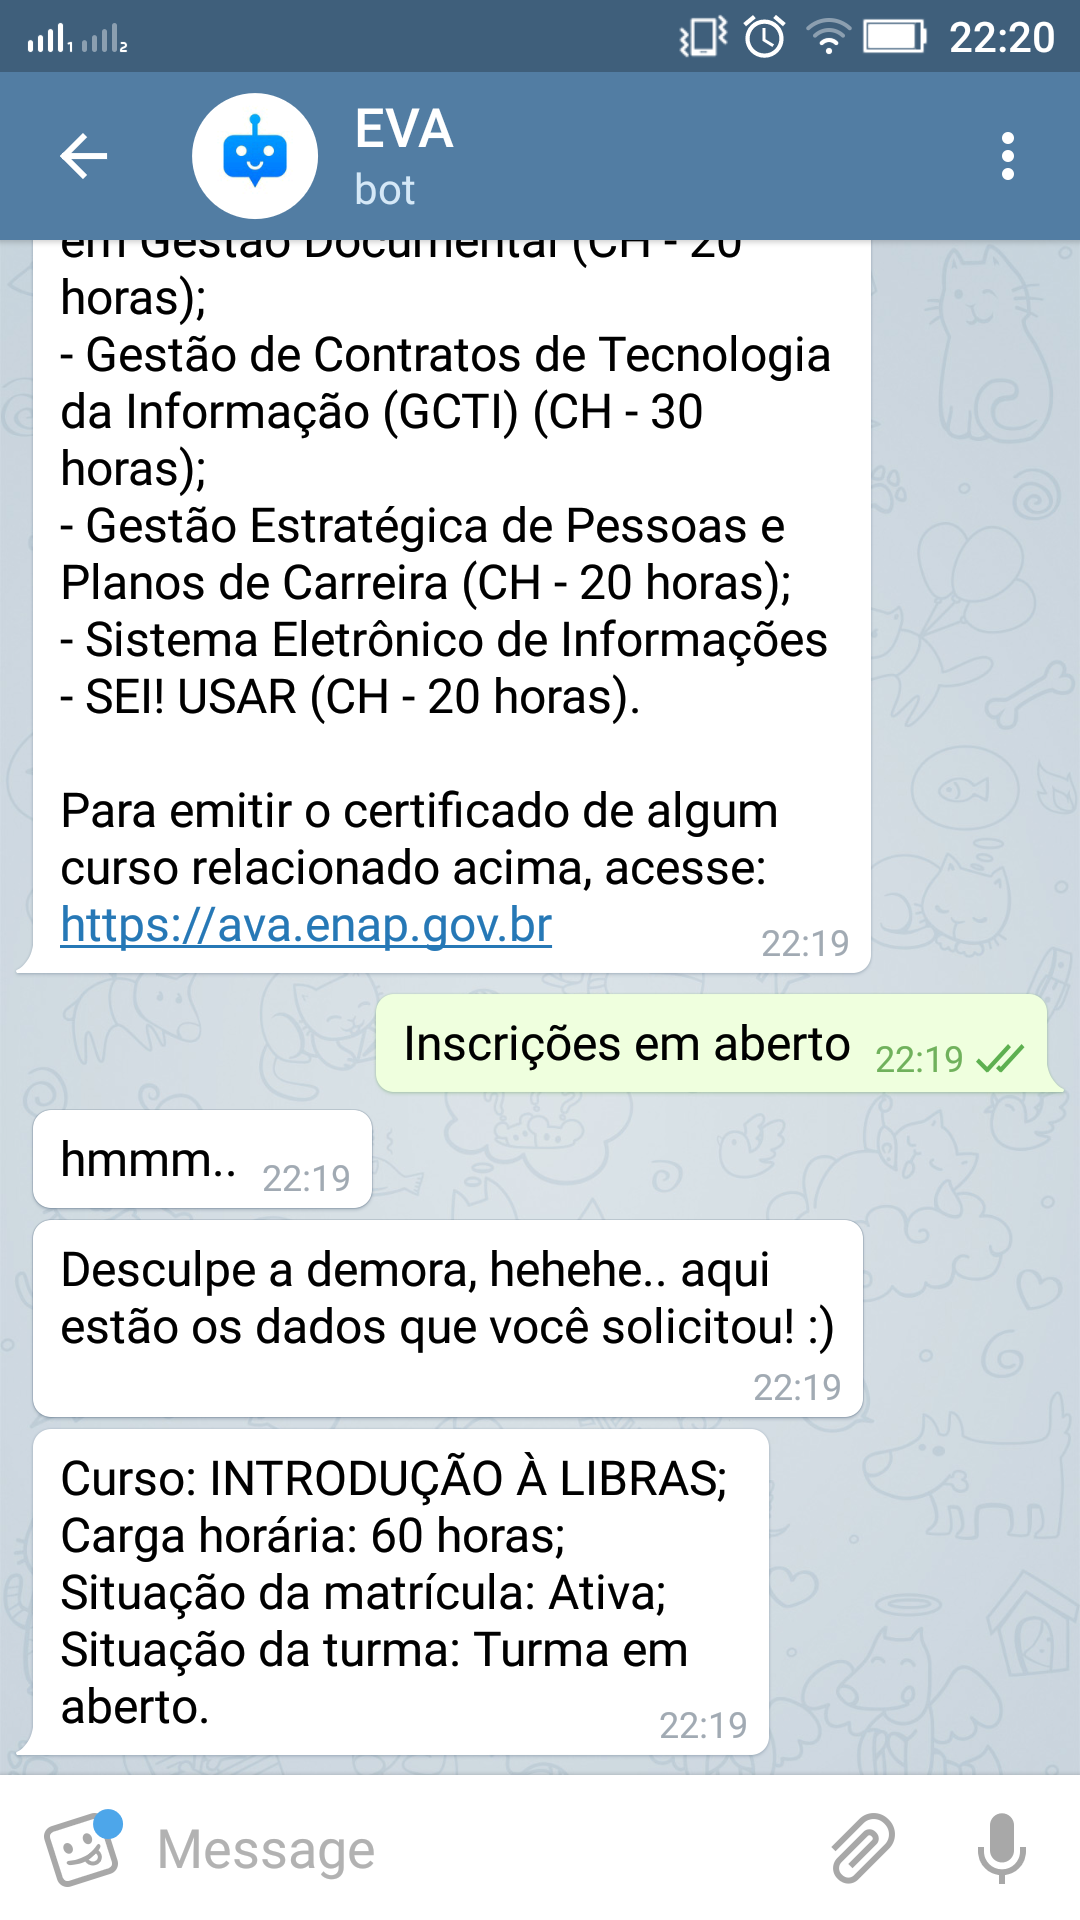
\includegraphics[width=0.2\linewidth]{src/imagens/apresentacao-cursos-aberto.png}
    \caption{EVA - Visualizando inscrições de cursos abertos} Fonte: Elaborado pelo autor (2018)
    \label{cap:04:fig:apresentacao-inscricoes-aberto}
\end{figure}

\section{Desvinculação}

A qualquer momento, se for da vontade do aluno, ele poderá se desvincular do sistema de EVA, apenas enviando uma simples mensagem de texto, demonstrado na Figura \ref{cap:04:fig:apresentacao-logout}.

\begin{figure}[htb!]
    \centering
    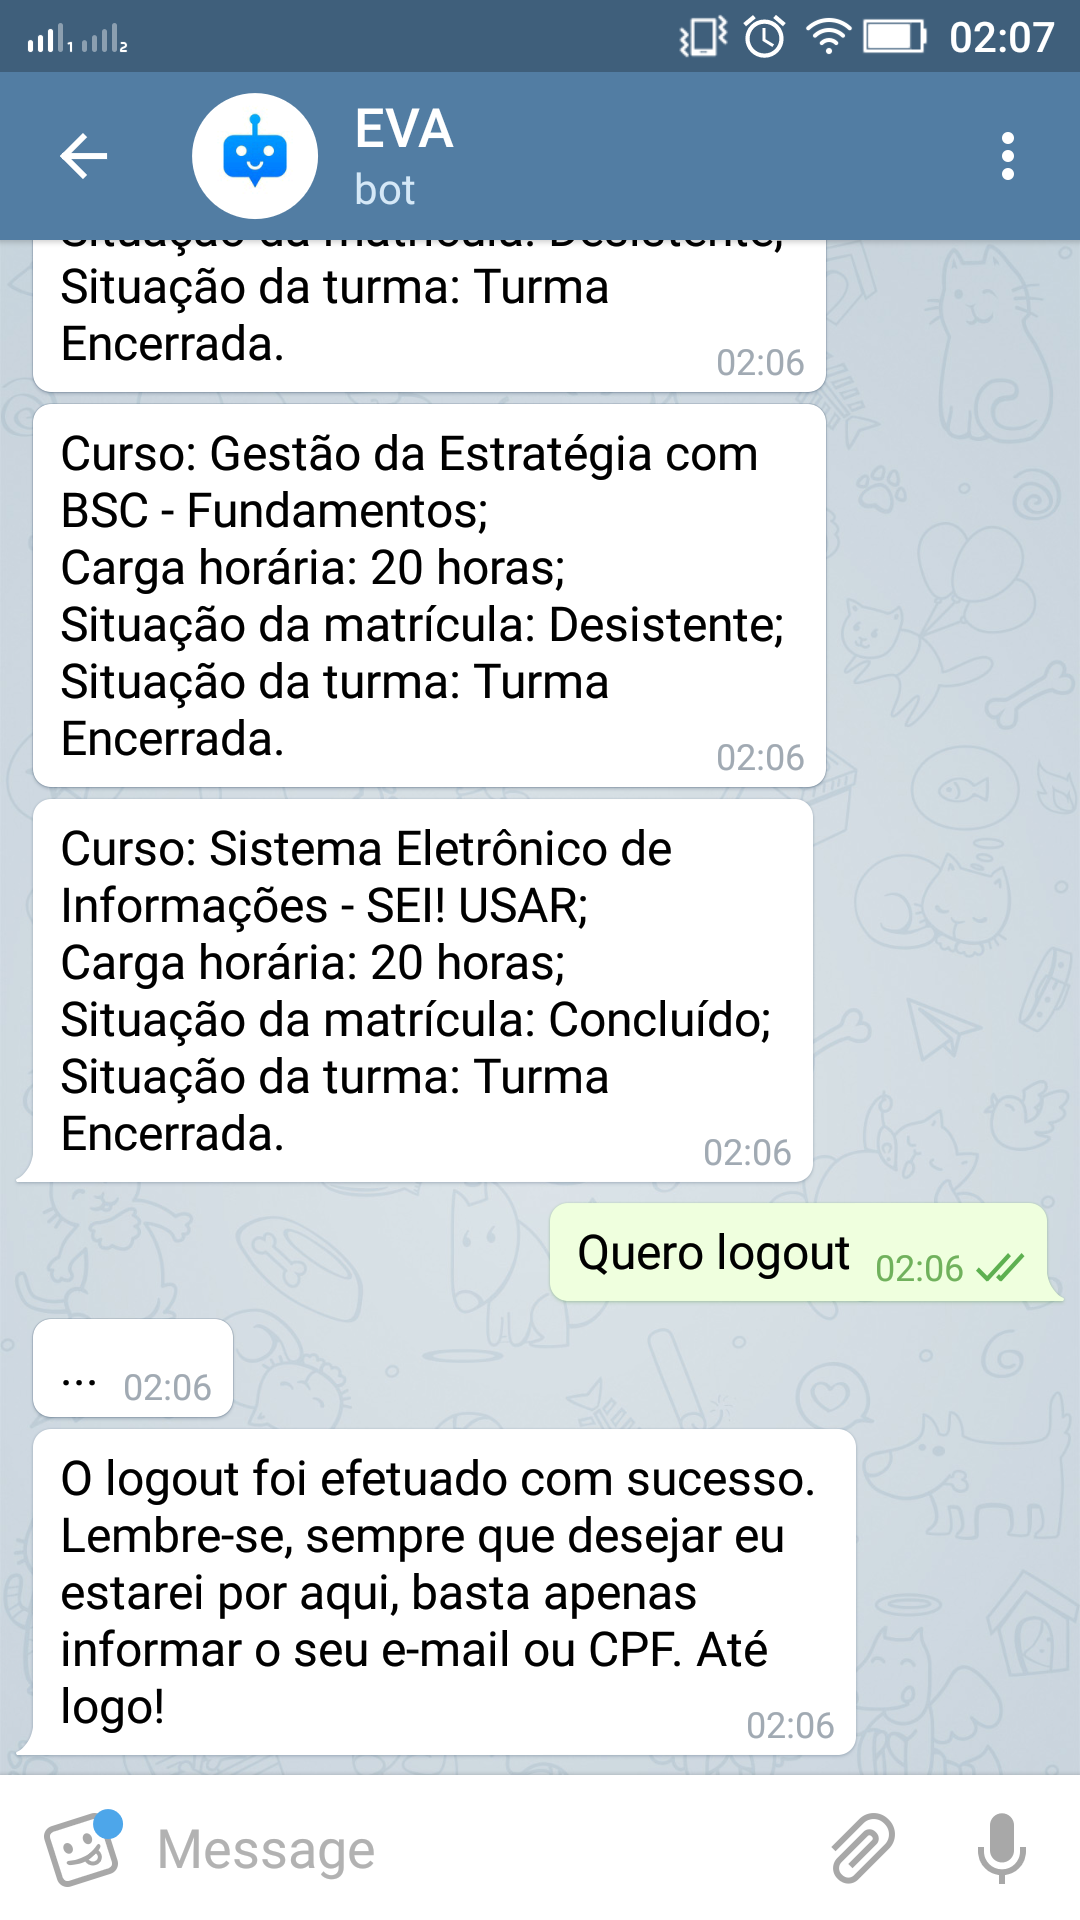
\includegraphics[width=0.2\linewidth]{src/imagens/apresentacao-logout.png}
    \caption{EVA - Logout} Fonte: Elaborado pelo autor (2018)
    \label{cap:04:fig:apresentacao-logout}
\end{figure}